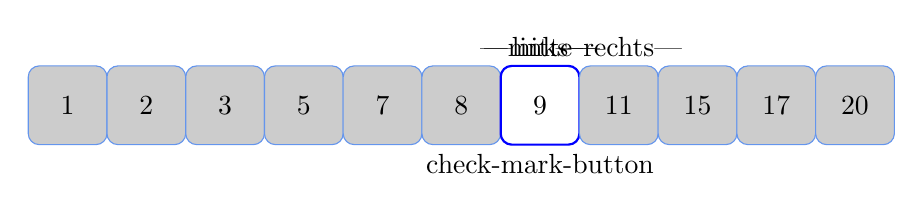
\begin{tikzpicture}
\node[draw=CornflowerBlue, fill=Black!20!White, rounded corners, minimum width=1cm, minimum height=1cm] at (0, 0) {1};
\node[draw=CornflowerBlue, fill=Black!20!White, rounded corners, minimum width=1cm, minimum height=1cm] at (1, 0) {2};
\node[draw=CornflowerBlue, fill=Black!20!White, rounded corners, minimum width=1cm, minimum height=1cm] at (2, 0) {3};
\node[draw=CornflowerBlue, fill=Black!20!White, rounded corners, minimum width=1cm, minimum height=1cm] at (3, 0) {5};
\node[draw=CornflowerBlue, fill=Black!20!White, rounded corners, minimum width=1cm, minimum height=1cm] at (4, 0) {7};
\node[draw=CornflowerBlue, fill=Black!20!White, rounded corners, minimum width=1cm, minimum height=1cm] at (5, 0) {8};
\node at (6,0) [rounded corners, minimum width=1cm, minimum height=1cm, draw=blue, thick] {9};
\node[draw=CornflowerBlue, fill=Black!20!White, rounded corners, minimum width=1cm, minimum height=1cm] at (7, 0) {11};
\node[draw=CornflowerBlue, fill=Black!20!White, rounded corners, minimum width=1cm, minimum height=1cm] at (8, 0) {15};
\node[draw=CornflowerBlue, fill=Black!20!White, rounded corners, minimum width=1cm, minimum height=1cm] at (9, 0) {17};
\node[draw=CornflowerBlue, fill=Black!20!White, rounded corners, minimum width=1cm, minimum height=1cm] at (10, 0) {20};
\node[above] at (6, 0.5) {\lstinline|links|};
\node[above] at (6, 0.5) {\lstinline|mitte|};
\node[above] at (7, 0.5) {\lstinline|rechts|};
\node[below] at (6,-.5) {\emoji{check-mark-button}};
\end{tikzpicture}
